% enginnering.tex

\documentclass[UTF8,10pt]{report}

%% 导言区,一般用于加载宏包
% 目录
\usepackage[titles]{tocloft}
% 引入中文
\usepackage{ctex} 
% 超链接
\usepackage[colorlinks,linkcolor=blue]{hyperref}
\usepackage{url}
% 引用
\usepackage{cite}
% \usepackage{natbib}
% 图片
\usepackage{graphicx}
% 数学
% 矩阵
\usepackage{mathtools}
\usepackage{amssymb}
\usepackage{amsmath}
\usepackage{arydshln}
% 嵌入代码
\usepackage{listings}
\usepackage{listings-ext}

% 给方程,图片,表格编号,section可能换成chapter
\renewcommand{\theequation}{\arabic{section}-\arabic{equation}}
\renewcommand{\thefigure}{\arabic{section}-\arabic{figure}}
\renewcommand{\thetable}{\arabic{section}-\arabic{table}}

\setlength{\baselineskip}{1.5em} % 行间距
\setlength{\parskip}{1.0ex} % 段间距
\setlength{\parindent}{0pt} % 段落缩进

% 文档开始
\begin{document}
%-----使用封面代替
%-----封面
\begin{center}
    \quad \\
    \vspace{0cm}
    \hspace{0cm}\Large{软件工程实践手册} \\
    \small{整理技术点,累积知识点,记录知识点} \\
    \hspace{0cm}\Large{李美杰} \\
    \hspace{0cm}\small{2019.9.23}
    \clearpage
\end{center}
%-----

%-----留白
\thispagestyle{empty}
\clearpage
%-----

%-----目录
\tableofcontents
\clearpage
%-----

% 代码区域样式
\lstset{
    language=C,
    numbers=left,
    frame=box
}

%-----正文
\clearpage
\part{Software Architecture}

\chapter{总思想}
软件架构是软件发展的必然之路,从最初开始的简单计算,花费那么大的精力来做计算,但是都是一步步来验证计算,
软件分层思想是软件发展的基础思想,这样就能保证在之前的基础上进行替换改进,能看到好的软件架构是能保证很多错误,
避免工程上的实现。


\section{网页开发}

\subsection{前后端分离}
前后端分离是发展趋势产生的,新业务发展,如3D,VR,Image,Computing,webGL等的产生,同时服务器面对的数据也是
几何级增加,为减少服务器方面的压力,同时利用终端设备的计算力。

前后端分离的好处在于各种业务独立发展,后端以稳定,性能,安全,存储等业务为核心,强调稳定,承受能力,数据处理与
环境干净;而前端注重效果,数据渲染等。

前后端分离后,平台无关化得到支持,网页,移动断,手机,LOT等,同时对团队更好,耦合性更低。随着与硬件无关的编程语言
发展迅速,如WebAssembly,Rust等必然产生前后端分离的需求,把服务器的压力全部限制在数据提供和反馈以及验证上,其他部分
都可放在前端。

\subsection{RESTful}
REST是Representational State Transfer的缩写,是目前互联网软件架构,它具备结构清晰,符合标准,易于扩展。
REST这个词是Roy Thomas Fielding在他2000博士论文中提出的。在前后端分离的基础上,前后端的交互只体现在API-server
上,即前后端只通过API来传输请求数据,只处理有效数据。


\section{工程方法}

\subsection{软件分层}
分层这个概念,是在整个计算机体系中是非常显而易见的的,这样保证每个阶段的发展是独立的,比如编程语言发展
肯定快于CPU的发展,必须抽象隔离开,每一层都在下一层的基础上发展,又同时为上一层服务。

\subsubsection{模块化}
工程方案小而美不是指代码量少,而是指规则,用最少最简单明了的规则制定出最容易遵守,最容易理解的
开发规范或工具,分而治之是软件工程中的重要思想,而模块化是最具体的方案。

\textbf{前端是一种技术问题较少,工程问题较多的软件开发领域,如大体量,多功能,多页面,多状态,多系统;
大规模:多人甚至多团队合作开发;高性能:CDN部署,缓存控制,同步异步加载等}

\subsubsection{组件}
component,是一个很泛的概念,就是软件复用的意思

\subsubsection{插件}
插件是一个很泛的概念,在软硬件中都存在的概念,这里只分析软件中的概念。

\textbf{插件与宿主程序的依赖关系}
\begin{itemize}
    \item {由外而内:内部需要其他模块,如ActiveX,Plugin方式提供服务}
    \item {由内而外:内部给了接口,外部新功能的添加,如Addon,Extension等}
\end{itemize}

\textbf{插件的完整性}
\begin{itemize}
    \item {可执行:宿主程序调用执行得到结果}
    \item {不可执行:如提交一个新的shader代码到程序内部,渲染不同的结果}
\end{itemize}

\subsubsection{中间件}
middleware,中间件是将业务逻辑与底层逻辑解耦的一种方式,就像设备之间的接口一样,确保两端各自独立,中间件
就沟通两端的。在大型集成项目中使用的一种灵活管理形式,是任意组合组件模型化的高效形式,使得整个业务可以分
模块并行开发。如果以某种标准的协议为接口的组件就可以任意组合成一个软件的一部分。体现在两个方面:
\begin{itemize}
    \item {上下页面分层}
    \item {层与层之间的解耦}
\end{itemize}


\subsection{敏捷开发}
核心就是迭代开发,每一次迭代都进行严格的执行顺序:
\begin{itemize}
    \item {requirements analysis, 需求分析}
    \item {design,设计}
    \item {coding,编码}
    \item {testing,测试}
    \item {deployment/evaluation,部署和评估}
\end{itemize}


\section{SOLID}

SOLID是一系列设计原则,帮助组织函数和类以软件具有robust鲁棒性,maintainable可维护性,
flexible灵活扩展性。

\subsection{Single Responsibility}
单一职责原则,一个类或函数只有应该只有一个目的,把对象划分成较小粒度,以达到对象的可复用性。

\subsection{Open-Closed}
开放封闭原则,Uncle Bob称为面向对象设计中最重要的原则,它指软件应该对扩展进行开放,对修改进行关闭。

通过接口或抽象类向外提供不同的策略,具体的策略由具体的类来实现。这样策略分离于具体细节,
保证了软件的松组合,同时高层的组件保护了底层组件的改变不受影响。

\subsection{Liskov-Substituion}
里氏替换原则,Barbara Liskov说\textbf{Let f(x) be a property provable about objects x of type T.
Then f(y) should be true for objects y of type S where S is a subtype of T.}

违背里氏替换原则的就是菱形(钻石)继承,子类通过父类调用祖类的方法时不能确定是那个的。

\subsection{Least Knowledge}
最少知识原则,指一个软实体应当尽可能少的与其他实体发生相互作用,软体是一个广泛的概念,不仅包括对象,还可指
系统,类,模块,函数,变量等。

减少对象之间的交互,不让这两个对象直接建立相互关系,因为那样就需要维护彼此的关系。把维护关系的任务交给
第三者,来承担对象之间的通信作用。

如将军需要挖掘一些散兵坑,将军与士兵的关系不是直接关系,就会出现这样的逻辑,将军通知上校,让上校叫来少校,
然后让少校叫来上尉,让上尉叫来一军士,让军士唤来一士兵,命令士兵挖掘散兵坑。
\begin{lstlisting}
    general.getColonel(c).getMajor(m).getCaptain(c)
        .getSergeant.getPrivate(p).digFoxhole();
\end{lstlisting}
维护这种关系会导致逻辑非常复杂。

\subsection{Interface Segregation}
接口隔离原则,阻止类依赖那些不是必须的一切

\subsection{Dependency Inversion}
依赖倒置原则,抽象不应该依赖细节,细节必须依赖抽象。\textbf{Abstractions should not depend on details,
Details should depend on abstractions.}

\section{Onion Architecture}
洋葱架构, Wade Waldron,其中最主要的概念是依赖,外部层能够访问内部的层,而内部层对外部的层一无所知。

\subsection{Core}
核心层是与领域或技术无关的基础架构块,包含一些通用的构件块,不包含任何技术层面的概念

\subsection{Domain}
领域层是定义业务逻辑的地方,每个类的方法都按照领域通用语言中的概念进行封装命名。对领域层的控制是通过API层
进行操作的。这种方式保证了应用程序的可移植性,在不丢失任何业务逻辑的情况下替换掉整个技术的实现

\subsection{API}
API层是领域层的入口,应该仅仅向外界暴露不可变的对象,以避免开发者通过暴露的对象获得对领域层的访问,或修改行为。
从API层开始编码工作,每个方法就是一个骨架,对应一个高层的功能性测试,随后添加逻辑层,以此驱动领域层的编码实现。

\subsection{Infrastructure}
基础架构层是最外部的一层,它包含了对接各种技术的适配器,如数据库,UI和外部服务等。

\chapter{CPU}

\section{Byte Order}

字节的顺序

\begin{description}
    \item [LSB] \text{least significant bit,最低位放在第0位}
    \item [MSB] \text{most significant bit,最高位放在第0位}
    \item [big-endian] \text{first byte(MSB),...,last byte(LSB)}
    \item [little-endian] \text{first byte(LSB),...,last byte(MSB)}
\end{description}

CPU有两个特色的\textbf{位处理指令},是硬件层内置,效率很高的。
\begin{itemize}
    \item {BSF, 前向位扫描}
    \item {BSR, 反向位扫描}
\end{itemize}

\section{Register}
寄存器
CPU 只负责运算,不负责存储数据,是LOAD-COMPUTE-SAVE原语模型。从内存中LOAD数据到CPU,执行计算,
完成后再SAVE回内存,而CPU的效率远高于内存,为解决LOAD和SAVE耗时,CPU自带了寄存器register来缓存,这样CPU优先
从register中获取数据,再由register与内存交换数据。
\newline
\textbf{register相比内存,是没有地址概念的,它们是通过自己的名称,CPU直接对名称进行操作的}
\newline
在Intel X86早期时,只要8个寄存器,\textbf{EAX,EBX,ECX,EDX,EDI,ESI,EBP,ESP},除ESP有特定用途(保存当前的stack栈的地址)
,其他7个是通用性寄存器。现在已经扩展到64位,特定领域的有更高的。 

\section{内存模型}
寄存器个数有限,更多的数据还是存在内存中。程序运行时,操作系统给程序分配一段内存(计算机物理内存可能很大,对不同
程序都要分配一段逻辑内存,保证每个程序都得到同样的对待)来存储程序和数据。
\newline
这段内存有起始地址和结束地址,如0x1000到0x8000.从低地址往高地址,有几个区域,分别为
\subsection{code area}
代码区,一般是只读区域,存储程序的源代码的二进制形式(即汇编的代码,CPU指令的二进制值指令,每条指令包含操作码,
操作对象或对象地址的引用)。
\newline
\textbf{曾经在我心中的,关于条件分支代码的执行,一直没有明白,总觉得要是这次执行true,下次执行false,那怎么来
保存这种组合的呢?让我困惑多年的不解之谜,原来就是在这里,所有代码都对应着CPU的执行,总是一遍又一遍的执行相同的
代码,从这个位置跳转到那个位置进行执行,循环递归下去至永远}
\newline
这些操作对象可能是
\begin{itemize}
    \item {立即数,直接存在代码区,如具体的数字5}
    \item {全局数据,在stack中分配空间存储,然后引用该数据的地址}
    \item {数据区,代码中引用的是它们的地址}
\end{itemize}

\subsection{data area}
由操作系统根据代码区创建的区域,与内存相关的操作由操作系统申请与释放。
\begin{itemize}
    \item {BSS-Block Started by Symbol, 静态内存分配,程序一开始清零的区域,运行期可动态改变;是全局变量未初始化
    ,以占位符的形式存在,未分配空间,仅记录数据的大小空间
    }
    \item {initial global data, 初始化全局变量,只执行一次}
    \item {static data, 全局,局部的静态变量,字符串,其中关于字符串常量是存在常量区还是stack区域,不同的编译器实现是有差异的}
\end{itemize}

\subsection{heap area}
向上增长,分配地址越来越大,由程序员分配和释放。

\subsection{stack area}
向下增长,分配地址越来越小。由系统自动分配,包括函数的参数值,局部变量等,执行完成后自动释放。

\subsection{argument area}
命令行参数区域,存放命令行参数和环境变量的值。

\subsection{编程语言模型的内存布局}
很多编程语言模型的内存布局是其性能高低的一个重要参数,C是堆栈结合,C++为了抽象,把对象的内存布局弄得较复杂,特别是多态的引入。
而想Java或其他语言,有GC的,基本都是在堆上的内存申请。
rust能到达C的性能,是满足了零抽象,不像C++那样有虚函数的开销,实用性得到满足了。

\section{Cache}

多核CPU有多级缓存,有关的一些特征,了解这些细节,对写出来的代码的性能影响是非常大的。
写的代码逻辑符合缓存机制,那速度是才是硬件层的,如果与缓存机制存在冲突,那速度就是非常糟糕的,可以慢如蜗牛。

\begin{description}
    \item [L1] \text{L1级缓存有两种,指令和数据缓存,后面的缓存不区分指令和数据}
    \item [位置] \text{L1和L2在第一个CPU中,L3是所有CPU共享}
    \item [速度] \text{离CPU越近,速度越快,L1 $>$ L2 $>$ L3 $>$ 内存 $>$ 硬盘}
    \item [耗时] \text{L1要4个CPU时钟周期存取,L2是11,L3是39,RAM是107}
\end{description}

缓存的目的就是把数据加载到离自己近的的位置,数据从内存到L3,再到L2,再到L1,最后到寄存器进行计算。造成这样的原因是物理与实践技术客观因素决定的。
这样引入两个问题,缓存的命中率和缓存的一致性。

\subsection{Cache Line}

缓存是一块块加载的,主流的64位是一次性加载64 bytes,嵌入式是32bytes或更低,游戏主机是128bytes。
L1有32kb/64b = 500个cache line。从内存到cache拷贝数据的过程是叫做CPU Associativity。它是因为使用的
数据结构N-Way关联,其他关系如下图所示
\begin{center}
    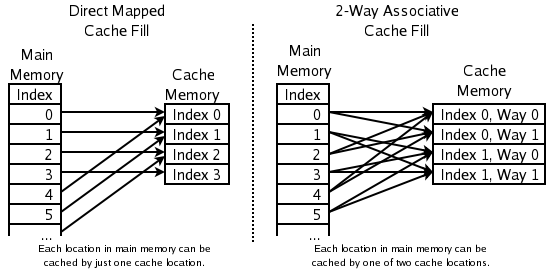
\includegraphics[width=0.8\textwidth]{images/cache-associative-fill-both.png}
\end{center}
主流的Intel是L1有32KB,8-Way,Cache Line是64bytes,于是有
\begin{enumerate}
    \item \text{cache line有32KB/64B=512条}
    \item \text{每一Way有512/8=64条cache line}
    \item \text{每一Way有64x64=4096bytes内存数据}
\end{enumerate}
为了方便索引地址,编码如下
\begin{itemize}
    \item \text{tag:每条cache line有24bit的物理地址}
    \item \text{index:每一Way的索引$2^6=64$,刚好索引每一Way的地址}
    \item \text{offset:每一Way中的cache line的偏移量}
\end{itemize}
\begin{center}
    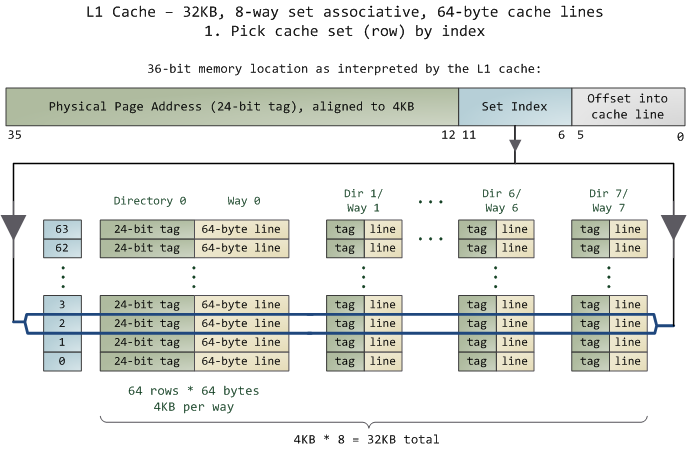
\includegraphics[width=0.8\textwidth]{images/L1CacheExample.png}
\end{center}
注意L1可以映射的内存地址是$2^36=64GB$,这样是解决了命中率的问题,还有Perfetching一些预测技术,可以一次性不止
64bytes的大小。

\subsection{一致性}

把数据从寄存器写出去产生的一致性问题,有两种策略

\begin{itemize}
    \item \text{Write Back, 只更新到cache,然后flush到内存上}
    \item \text{Write Through,更新到cache和内存上}
\end{itemize}

目前主流的还是Write Back策略,毕竟写入内存太耗时了。
现在假设一个数据X在CPU第0核的cache上更新了,其他核对于数据X也要更新,这就是一致性问题。
在CPU硬件层有两种方案:

\begin{itemize}
    \item [Directory] \text{存储全局信息,更新时同时检查哪些需要更新}
    \item [Snoopy] \text{以总线技术,类似广播形式,更新到所有的cache中的数据}
\end{itemize}

Directory属于中心式,会有性能瓶颈,目前都使用Snoopy总线设计方案。实现这些细节需要一些协议.

\subsubsection{MESI}

表示Modified已修改,Exclusive独占的,Shared共享的,Invalid无效的。

\begin{center}
    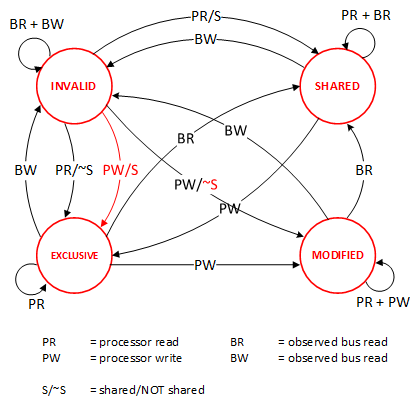
\includegraphics[width=0.8\textwidth]{images/MESI.png}
\end{center}

\begin{tabular}{|c|c|c|c|c|}
    \hline
    \hbox{当前操作} & CPU0 & CPU1 & Memory &  \hbox{说明} \\ \hline
    \hbox{1) CPU0 read(x)} & \hbox{x=1(E)} & & \hbox{x=1} & \hbox{只有一个CPU,状态是Exclusive} \\ \hline
    \hbox{2) CPU1 read(x)} & \hbox{x=1(S)} & \hbox{x=1(S)} & \hbox{x=1} & \hbox{两个CPU读取,状态为Shared} \\ \hline
    \hbox{3) CPU0 write(x,9)} & \hbox{x=9(M)} & \hbox{x=1(I)} & \hbox{x=1} & \hbox{变量改变,CPU0是Modified,CPU1是Invalid} \\ \hline
    \hbox{4) flush to memory} & \hbox{x=1(E)} & \hbox{x=1(E)} & \hbox{x=9} & \hbox{状态不变} \\ \hline
    \hbox{5) CPU1 read(x)} & \hbox{x=9(S)} & \hbox{x=9(S)} & \hbox{x=9} & \hbox{变量同步更新,状态为Shared} \\ \hline
\end{tabular}

AMD使用是MOESI,Intel使用的是MESIF。

\subsubsection{MOESI}

Owner宿主

\subsubsection{MESIF}

Forward



\clearpage

\part{programming language}
编程语言是工具,是服务于软件工程的最基本的工具。针对不同的需要才会产生对应的语言工具,
没有一种语言是万能的,是通用的,每一门编程语言都是特定领域的特定产物。

\section{通用概念}

\subsection{异常}
异常,一般指程序运行期发生的非正常情况,一般是不可预测的,如内存不足,除零等。
它与软件编程思想、编程语言的发展是与时俱进的,核心思想就是把功能代码模块与系统中
可能出现的错误处理代码分离开来,以此达到代码组织结构更加美观、逻辑清晰,
且对软件系统长时间运行提供保障.

\subsubsection{goto}
goto本质上是对异常处理的思维,也是最初最原始的方法,有点很多,这里列出它的劣势:
\begin{itemize}
    \item {在函数的局部作用域内跳转}
    \item {破坏程序的结构化设计,代码难以测试}
\end{itemize}

\subsubsection{setjmp}
c语言中提供了setjmp和longjmp函数,是结构化异常的基础,首先设置一个跳转点setjmp可以实现,
然后在代码的其他任意地方调用longjmp函数跳回到这个点上。
\newline
支持这些功能的是有一个异常结构体,用于保存当前程序的现场。
\begin{lstlisting}
    typedef struct {
        unsigned j_sp;
        unsigned j_ss;
        unsigned j_flag;
        unsigned j_cs;
        unsigned j_ip;
        unsigned j_bp;
        unsigned j_di;
        unsigned j_es;
        unsigned j_si;
        unsigned j_ds;
    }jmp_buf;
\end{lstlisting}
setjmp和longjmp都与这个结构有关,setjmp还是一个能返回两次的函数,第一次是调用时,第二次是longjmp时。
\begin{lstlisting}
    #include <stdio.h>
    #include <setjmp.h>
    jmp_buf jumper;
    int div(int a, int b) {
        if (b == 0) {
            longjmp(jumper, -3); // the setjmp 
            //call second with the second parameter
        }
        return a / b;
    }
    int main(int argc, char **argv) {
        // longjmp会调用的位置
        int retcode = setjmp(jumper); 
        if (retcode == 0) {
            printf(" div result is %d\n", div(2, 0));
        } else if (retcode == -3) {
            printf(" divide by zero");
        } else {
            printf(" unhandled error case");
        }
        return 0;
    }
\end{lstlisting}

\subsubsection{全局处理}
C++,Java等高级语言的异常处理机制,是借助全局进行处理,并没有专门提供能够有效区分正常逻辑和错误逻辑的语法,
所有的非正常都当作异常处理,且还会带来较大的性能开销。

\subsection{调用约定}
函数调用约定,是对函数调用的一个约束和规范,包含
\begin{itemize}
    \item {函数参数的压栈顺序}
    \item {由调用者还是被调用者把参数弹出栈,调用者自己清理堆栈上的参数的,
    可以实现可变参数列表功能}
    \item {产生函数修饰名的方法}
\end{itemize}

\subsubsection{cdecl}
C declaration,C声明是C语言的一种调用约定,事实上的标准。参数按照从右向左的顺序
依次压栈,调用者负责清栈。不同编译器不同平台实现的细节上是存在差异的。可编译成对应
的汇编代码来分析。函数名加一前缀(下划线字符)。

\subsubsection{pascal}
基于Pascal语言的调用约定,参数从左向右入栈.被调用者负责在返回前清栈.

\subsubsection{stdcall}
由微软创建的调用约定,是Windows API的标准调用约定。它结合了cdecl和Pascal两者优势,
参数从右向左入栈,被调用者负责清栈。编译后函数名添加后缀@length,length是传递函数参数
所占的栈空间的字节长度.

\subsection{语言特性}
特性,即概念的描述方式,王银在他的文章《如何掌握所有的程序语言》中描述的那样:
\textbf{如果你不能用一种语言里面的基本特性写出好的代码,那你换成另外的一种语言也
无济于事。是否能写出好的代码在于人,而不在语言。如果你心中没有清晰简单的思维模型,
你用任何语言特性表述出来的都是一堆乱码。}

而每个语言特性尽量从古老语言中追溯,新语言的特性完全是封装了一个新的概念在其上,编程
语言比自然语言简单清晰,也更加严谨和形式化。所以不要想着用尽语言提供的特性,而是使用
经过千锤百炼的特性才能保证稳定性。

\subsubsection{指针}
在C,C++语言中,指针是一个很灵活的方法,但不是所有语言都有这种特性,也不适合一些语言。
它们使用指针是因为它们可以直接与硬件进行沟通,而在现代化的快速应用中,很多软件都是建立在
一个抽象层上面进行开发的,就是为了确保与硬件无关,所以这些语言根本不需要指针这种概念,如
Java就没有指针概念!因为它是建立在C,C++编写的应用上面的一种抽象语言。

\subsubsection{mutable与immutable}
\textbf{mutable}与\textbf{immutable}这两个概念是函数式编程语言中是很基础的概念,它们对变量加强了说明,
是在语义上进行改进的语言。也是区分静态类型与动态类型语言的一个指标,静态类型语言是要严格区分的!

C++中默认是可变的,不可变的需要加上const,这是比较反常的。这也是C/C++最令人痛苦的过程就是,在很多地方的默认
是让人不注意的,特别是学习过程中没有入坑解决这些问题,是很难做到条件反射的,总是会产生错觉!

在Rust这样的语言中,为确保类型安全,明确了语言的语义,在语义上通过编译器来保证逻辑上的清晰,既有函数式风格,
也有系统编程语言的能力,避免存在歧义的语句存在,每一条语句都需要明确到位。

\subsubsection{constant}
常量,在它的范围内scope只声明一次,不可更改的变量。
常量表达式,就是在编译期可计算的值,而不是运行期中计算得到的值。

\subsubsection{函数}
特性有如下特性:
\begin{itemize}
    \item {函数是一阶值,First-class valuue, 即函数可以作为另一个函数的返回值或参数,也可作为变量值}
    \item {函数可以嵌套定义,即一个函数内部可以定义另一个函数}
    \item {可以捕获引用环境值}
    \item {允许定义匿名函数}
    \item {把引用环境和函数代码组成一个可调用的实体}
\end{itemize}
根据不同的需求,可以变化为
\begin{itemize}
    \item {lambda,匿名函数}
    \item {Closure,闭包,又称词法闭包lexical closure或函数闭包function closure。
    是由支持高价函数特性的语言技术,是实现静态作用域的一种方式,将函数与声明时的作用域保存
    下来,在被调用时的有效作用域是在声明时的,而不是调用执行时的}
\end{itemize}

\subsubsection{inline}
内联,短小的函数不存在函数调用的开销,是因为现代编译器都能自动把小函数inline到被调用的地方。
早期的C语言编译器里,宏就是有这么一个功能,替换小函数,这也是大量使用宏的原因。

\subsubsection{FFI}
Foreign Function Interface, 是指与其他语言交互的接口,现实中的程序基本没有单语言的软件啦!
跨语言调用就成了一门语言的必然趋势,常用方法有两种
\begin{itemize}
    \item {将函数做出一个服务,通过进程通信IPC或网络通信协议RPC,RESTful等方式进行,至少需要两个进程}
    \item {直接FFI调用,直接将其他语言接口内嵌到语言中进行调用}
\end{itemize}
大多数属于兼容C ABI的实现。

\subsubsection{生成器}
生成器generator是一种特殊的迭代器,是一个函数,能多次返回的函数,即遇到yield就是返回,下次执行函数时从上一次yield的地方继续执行,这种机制就称为生成器。

yield关键字有两点作用
\begin{itemize}
    \item {保存当前运行状态,断点处,然后暂停执行,将生成器函数挂起}
    \item {将yield关键字后面表达式的值作为返回}
\end{itemize}

\subsubsection{协程}
协程是指具有这些函数
\begin{itemize}
    \item {彼此间有不同的局部变量,指令指针,但任共享全局变量}
    \item {可以方便挂起,恢复,并且有多个入口和出口点}
    \item {多个协程间表现为协作运行,同一时刻只能有一个协程运行,即无法并发,不含多线程情况}
\end{itemize}

\subsubsection{多态}
在编程语言和类型论中,多态polymorphism指为不同数据类型的实体提供统一的接口。
多态类型polymorphic type可以将自身所支持的操作套用到其他类型的值上。

而据派发dispatch发生时间的不同,多态分为静态(编译时)和动态(运行时)。

C++中的虚继承就属于动态多态,它实现的方式是为继承类加入一个域vptr,指向vtbl。继承类调用方法时是先通过vptr到vtbl中找到函数再调用。
C++中的模板与重载是静态多态,在编译期完成模板展开,直接链接到对应的函数,消除了虚函数的开销。

Rust中引入的trait系统解决了C++中的缺点。


\subsection{编程范型}
The principal programming paradigms.\cite{TPPP}列出了编程范型。

\subsubsection{过程}

\subsubsection{结构化}

\subsubsection{面向对象}

\subsubsection{泛型}

\subsubsection{函数式}

\subsubsection{并发}

\subsubsection{分布式}

\subsubsection{DSL}
Domain Specific Language,领域编程语言,基于特定领域开发相关的编程语言。

\subsubsection{IDL}
interface description language, or interface definition language,
接口描述(定义)语言,是一种语言规范,用来描述组件的API。在跨语言,RPC方面上
大量应用。

\subsubsection{Glue code}
glue code language,胶水语言,

\section{计算机组织结构}
目前接触到的都是冯诺依曼体系结构的计算机,它也是现代计算机的产生的基础。
\subsection{CPU}
LSB-least significant bit最低位放在第0位,MSB-most significant bit,最高位放在第0位。
\newline
big-endian, first byte(MSB),...,last byte(LSB)
\newline
little-endian, first byte(LSB),...,last byte(MSB)。
\newline
CPU有两个特色的\textbf{位处理指令},是硬件层内置,效率很高的。
\begin{itemize}
    \item {BSF, 前向位扫描}
    \item {BSR, 反向位扫描}
\end{itemize}

\subsubsection{寄存器}
CPU 只负责运算,不负责存储数据,是LOAD-COMPUTE-SAVE原语模型。从内存中LOAD数据到CPU,执行计算,
完成后再SAVE回内存,而CPU的效率远高于内存,为解决LOAD和SAVE耗时,CPU自带了寄存器register来缓存,这样CPU优先
从register中获取数据,再由register与内存交换数据。
\newline
\textbf{register相比内存,是没有地址概念的,它们是通过自己的名称,CPU直接对名称进行操作的}
\newline
在Intel X86早期时,只要8个寄存器,\textbf{EAX,EBX,ECX,EDX,EDI,ESI,EBP,ESP},除ESP有特定用途(保存当前的stack栈的地址)
,其他7个是通用性寄存器。现在已经扩展到64位,特定领域的有更高的。 

\subsection{内存模型}
寄存器个数有限,更多的数据还是存在内存中。程序运行时,操作系统给程序分配一段内存(计算机物理内存可能很大,对不同
程序都要分配一段逻辑内存,保证每个程序都得到同样的对待)来存储程序和数据。
\newline
这段内存有起始地址和结束地址,如0x1000到0x8000.从低地址往高地址,有几个区域,分别为
\subsubsection{code area}
代码区,一般是只读区域,存储程序的源代码的二进制形式(即汇编的代码,CPU指令的二进制值指令,每条指令包含操作码,
操作对象或对象地址的引用)。
\newline
\textbf{曾经在我心中的,关于条件分支代码的执行,一直没有明白,总觉得要是这次执行true,下次执行false,那怎么来
保存这种组合的呢?让我困惑多年的不解之谜,原来就是在这里,所有代码都对应着CPU的执行,总是一遍又一遍的执行相同的
代码,从这个位置跳转到那个位置进行执行,循环递归下去至永远}
\newline
这些操作对象可能是
\begin{itemize}
    \item {立即数,直接存在代码区,如具体的数字5}
    \item {全局数据,在stack中分配空间存储,然后引用该数据的地址}
    \item {数据区,代码中引用的是它们的地址}
\end{itemize}

\subsubsection{data area}
由操作系统根据代码区创建的区域,与内存相关的操作由操作系统申请与释放。
\begin{itemize}
    \item {BSS-Block Started by Symbol, 静态内存分配,程序一开始清零的区域,运行期可动态改变;是全局变量未初始化
    ,以占位符的形式存在,未分配空间,仅记录数据的大小空间
    }
    \item {initial global data, 初始化全局变量,只执行一次}
    \item {static data, 全局,局部的静态变量,字符串,其中关于字符串常量是存在常量区还是stack区域,不同的编译器实现是有差异的}
\end{itemize}

\subsubsection{heap area}
向上增长,分配地址越来越大,由程序员分配和释放。

\subsubsection{stack area}
向下增长,分配地址越来越小。由系统自动分配,包括函数的参数值,局部变量等,执行完成后自动释放。

\subsubsection{argument area}
命令行参数区域,存放命令行参数和环境变量的值。

\subsubsection{编程语言模型的内存布局}
很多编程语言模型的内存布局是其性能高低的一个重要参数,C是堆栈结合,C++为了抽象,把对象的内存布局弄得较复杂,特别是多态的引入。
而想Java或其他语言,有GC的,基本都是在堆上的内存申请。
rust能到达C的性能,是满足了零抽象,不像C++那样有虚函数的开销,实用性得到满足了。

\section{编译器}
编译器的技术就是翻译人与机器的沟通,体现在两方面,一是工程化需要,需要大量的交流,不能简简单单的操作硬件来完成;
一是简化人的交流成本,特别在指定领域,快速的结果是推导前进的基础。

\subsection{概念}

\subsubsection{自举}
用低级语言先实现一个简单的编译器,然后用这个编译器的语言再去编写一个更高级的编译器.
新编译器就是旧编译器的扩展,这个过程称为自举.

\subsubsection{交叉编译}
不是每个设备都像PC这样便利,为其他设备进行软件开发的过程需要的技术。分两类
\begin{itemize}
    \item {\textbf{小设备},如嵌入式或手机,在PC上完成编译过程,把打包的二进制放入小设备内存中运行.
    本质就是 PC 运行小设备的编译器进行开发,这样避免掉小设备的内存、开发环境、效率等限制}
    \item {\textbf{跨平台},使用Linux编译一个程序,移植portable到window上.本质就是源设备上的编译器,
    具有生成目标设备上的机器代码的功能}
\end{itemize}

\subsubsection{JIT}
Just In Time,即时编译,混合了静态编译与动态解释,将频繁执行的代码编译成机器码缓存起来,对于执行一次的代码任然是
逐行逐条解释执行的技术。
\newline
\textbf{Method JIT},方法即时编译,如Java。主要的步骤如下
\begin{itemize}
    \item {跟踪热点函数,编译成机器码执行,并缓存}
    \item {非热点函数解释执行}
\end{itemize}
\textbf{Trace JIT}, 跟踪即时编译,如Lua,相比Method JIT,它不检测和优化热点函数,而是检测并优化热点跟踪或执行路径。

\subsection{GC}
Garbage Collection
\subsubsection{mark-and-sweep}
系统管理所有创建的对象,每个对象都有对其他对象的引用,root集合代表着已知的系统级别的对象引用。从root集合出发,就可以访问
到系统引用的所有对象,而没有被访问的对象就是垃圾对象,需要被销毁的,状态分为
\begin{itemize}
    \item {white,待访问状态,还未被gc访问到}
    \item {gray,待扫描状态,已被访问到,但它对其他对象的引用还未访问到}
    \item {black,已扫描状态,对象关联的都已访问到}
\end{itemize}
\begin{lstlisting}
    all object set white
    visit root set to  put gray set,
    make white to gray state 
    while gray set no empty {
        fetch object from gray set, object set black 
        for (obj in all object referenced by object) {
            if obj is white 
                obj from white to gray, 
                and add to gray set 
        }
    }
    for any object {
        if object is white {
            destory object 
        } else {
            set object white state
        }
    }
\end{lstlisting}

\subsection{BNF}
Backus-Naur Form巴科斯范式,用来描述计算机语言语法的符号集,是一种典型的元语言,它严格地表示语法规则,
且描述的语法与上下文无关的,它的扩展是ABNF 
\cite{ABNF}

\subsubsection{expression}
表达式在编程语言中代表一个可以返回值的语法单位,在不同语言中有不同的形式:
\begin{itemize}
    \item {函数式编程语言,大多数语句都是表达式}
    \item {命令式编程语言,一般将语句分成表达式和陈述句statement}
    \item {常量表达式,在BNF中属于终结符}
\end{itemize}

\subsection{工具}
Lex \& Yacc是一套生成语法的工具,可以快速方便成型。相对于手写的词法器,具有一定的优势。


\section{编译型语言}

\subsection{assembly}
老实说,汇编是没有学到家的,相当于熟悉了一遍它的常用语法,没有实战经验,最主要的是想
学的底层技术,并没有融会贯通于硬件层.
\newline
多年后(2019.6)才理解,微处理器是管理计算机的算术、逻辑、控制等,都有一套专门的指令码,在汇编中称为
opcode,操作码,操作码是二进制形式的,如00000011是加法指令,对应着的文本形式就是ADD,即\textbf{汇编语言是
二进制指令的文本形式,与指令存在一一对应的关系,把汇编的文本转换为二进制后就是CPU的指令码}。

\subsection{C}
C语言虽然是入门语言. 可是仅仅学了一些照本宣科的知识,没有体会实际中的技巧,更不用谈C中的那些奇淫技巧啦.
没有足够的机会去应用,就像屠龙之术一样,很多时候学的时候并没有讲得精髓,更多的是一些场面话语,
官方的教师描述的如此重要的一门语言,一门空谈过多的语言!
\subsubsection{struct}
c的struct的用法,很多技术,但是也容易有很多混淆的地方。
\begin{lstlisting}
    typedef struct tagS1 {
        int member;
    }S1;
    S1 s1; // 变量声明,等价于struct tagS1 s1;
    typedef struct {
        int member;
    }S2;
    S2 s2; // 变量声明
\end{lstlisting}

\subsection{Cplusplus}
C++引入一个核心概念ADT,Abstract Data Type.是为类型的属性和类型的操作方法提供了一个抽象
的描述,且不受特定的实现和编程语言的约束。C++使用class关键字来封装数据和函数方法。

\subsubsection{对象模型}
对象模型的发展有几个阶段,分别是

Simple Object Model,所有的member都不放在object中,只保存指向member的指针。这个模型
抽象得太理想,很容易理解,但实际中没有应用。

Table-driven Object Model,是为了对所有class的对象object都有一致的表达方式,让object
内含两个表格指针,分别指向
\begin{itemize}
    \item {member data table}
    \item {function member table}
\end{itemize}

C++的实际模型是继承了简单对象模型和表格驱动模型的优点,满足在空间和存取的时间效率,
缺点也存在,就是class内的一些改动就会导致需要重新编译,影响开发效率。模型结构大致如下:
\begin{itemize}
    \item {non-static data member, 都在class之内}
    \item {static data member,都在class之外}
    \item {function member都在class之外}
    \item {virtual function,与其他不同。每个class有多个指向virtual function的指针,都放在
    一个表格中,称为virtual table(vtbl),每个class内含一个指针指向这个virtual table, 这个指针
    称为vptr}
\end{itemize}

\subsubsection{成员函数}
构造函数,只在特定情况下会由编译器构建:
\begin{itemize}
    \item {class A中的member是class B的对象,B有默认构造函数,编译器会给A生成一个默认构造函数,
    用来调用成员class B的对象的初始化,其他member是不会自动初始化的,是程序员的负责对它们进行初始化。
    需要避免多个默认构造函数,使用inline}
    \item {class A的基类有默认构造函数,编译器会生成A的默认构造函数,以调用基类的默认构造函数来完成
    初始化。如果基类没有,编译器不会为A生成默认构造函数}
    \item {class A存在虚函数,编译器会默认生成构造函数,构造vtbl和vptr}
    \item {class A存在虚基类,编译器会生成默认构造函数,以初始化虚基类的vtbl}
\end{itemize}

拷贝构造函数,在以下情况下会由编译器生成,
\begin{itemize}
    \item {显示对class A进行初始化}
    \item {class A作为函数的参数}
    \item {函数返回一个class A}
\end{itemize}
位逐次拷贝,bitwise copy semantics。即class A中不存在class member对象时,拷贝就是对class
A中的每个bit进行拷贝,即POD(Plain Old Data),这时支持static initializtion,内存布局和对应的
C语言的struct布局相同。

\subsubsection{多态机制}
case这个概念是一种编译器指令,它只影响编译器如何解释指针指向的内存大小和内容。

\subsubsection{struct}
很多适合并没有弄明白C++中的struct和C中的struct的区别,听到更多的是以C++中的概念来理解。
\begin{lstlisting}
    struct S1 {
        int member;
    };
    S1 s1; // 变量声明
    struct S2 {
        int member;
    }S2; // S2直接成为一个变量啦
    S2.member = 1; // 还是全局的变量,直接访问内部
    typedef struct tagS3 {
        int member;
    }S3; // S3是一个结构体类型
    S3 s3; // 声明变量
    s3.member; // 必须先声明后使用
\end{lstlisting}

\subsubsection{value-category}
C++的表达式具有两个属性,一个是type,一个是value category,判断一个表达式的特征就是参考value-category
来确定的。

C++11之前,只有两类,lvalue和rvalue,即根据赋值符合的左右来区分,左值是表达式结束运算后
依然存在的持久对象,右值是表达式结束后就不再存在的临时对象。

C++11开始,引入了移动语义move semantic后,产生了语义上需要。\textbf{注意,计算机语言是计算机科学与语言学的
交叉科目,很多概念来自语言学内容}。先从自然语言中举个例子来说明
\begin{enumerate}
    \item {他是饭桶}
    \item {这是饭桶}
\end{enumerate}
上面两句话都有饭桶这个词,但是意思是不一样的,语法形式上相同的语句,却因代词不同结构完全无关。
说明一条语句不能仅靠词来确定,还需要整个句子的逻辑性,语义性。C++中也有类似的表达式:
\begin{enumerate}
    \item {vec = vect<int>()}
    \item {vec = another-vec}
\end{enumerate}
形式也是一样,但第一句的语义是表示移动赋值,第二句的语义表示复制拷贝一份。所以在C++11中,重新
定义了value categories:
\begin{itemize}
    \item {是否具有identity,即是否可以与另一个表达式进行比较,具有identity同一性的才具有比较
    的意义,如内存地址,堆栈上的变量都具有identity}
    \item {是否呈现移动的语义}
    \begin{itemize}
        \item {lvalue, 有identity且无移动语义}
        \item {xvalue,有identity且有移动语义}
        \item {prvalue,pure rvalue,无identity且有移动语义}
        \item {glvalue,有identity的表达式}
        \item {rvalue,有移动语义的表达式。如对象成员表达式,object.member,如果member是枚举或非
        静态成员函数,则object.member就是prvalue。因为枚举编译后是要给具体的数字,如5,成员函数
        在编译后是一个相对地址,本质上也是一个具体的数字,CPU使用这些数字时,是直接放在指令内部或
        寄存器中,不会放在内存中,即没有identity}
    \end{itemize}
\end{itemize}

\subsubsection{CRTP}
Curiously Recurring Template Pattern,奇异递归模板模式。1980年作为F-bound polymorphic
被提出
\begin{itemize}
    \item {静态的多态,无法动态绑定。CRTP强迫继承接口,可与Concept这个概念结合来理解}
    \item {多态的转换调用是在编译期时解决,而不是留到运行期处理,性能得到提高。CRTP起到了虚函数的效果,
    却无虚函数的开销,因为虚函数需要存储虚函数指针,调用时通过虚函数指针查找虚函数表进行调用}
    \item {std::enable\_shared\_from\_this针对std::shared\_ptr就是实例,WTL微软的轻量级窗体库}
\end{itemize}

\subsection{Rust}

\subsubsection{类型系统}
借鉴了Haskell的类型系统特性有
\begin{itemize}
    \item {没有空指针}
    \item {默认不可变}
    \item {代数数据类型}
    \item {高阶函数}
    \item {模式匹配}
    \item {trait和关联类型}
    \item {本地类型推导}
\end{itemize}
借鉴了C++的
\begin{itemize}
    \item {确定性析构}
    \item {RAII}
    \item {智能指针}
\end{itemize}
加上本身独有的特性
\begin{itemize}
    \item {仿射类型Affine Type,用来表达Rust所有权中的move语义}
    \item {借用,生命周期}
\end{itemize}

\subsubsection{生命周期}
很重要的概念就是生命周期,所有权和移动语义,借用概念。相比C/C++中的默认拷贝赋值,rust中不注意调用一下自己就没啦!
默认情况下是移动语义,很多时候要强调是借用,就像C的指针,C++的引用一样,使用起来时要注意这些基础的概念,是很容易
影响写代码的逻辑的。

struct中很重要的概念是生命周期,结构体中的每个字段都是完整的属于自己的,即每个字段的生命周期最终都不会超过
这个结构体。
\begin{lstlisting}
    struct A {
        attr1: i32,
        attr2: String,
    }
    struct RefBoy<'a> {
        loca:&'a i32,
    }
\end{lstlisting}
RefBoy的生命期一定不能比'a更长,即结构体里的引用必须要有显式生命周期,一个辈显式写出的生命周期的结构体,其自身
的生命周期一定小于等于其显式写出的任意一个生命周期。

\section{解释型语言}

\subsection{lua}
lua目前是没有标准的,是一门小语言,它的优势在于小巧,代码很少,足够到去全部理解,
用来学习是非常适合的,学习编译原理相关的知识,都可以通过它来一窥乾坤!

\subsection{Javascript}

\subsection{Typescript}

\chapter{assembly}
老实说,汇编是没有学到家的,相当于熟悉了一遍它的常用语法,没有实战经验,最主要的是想
学的底层技术,并没有融会贯通于硬件层.
\newline
多年后(2019.6)才理解,微处理器是管理计算机的算术、逻辑、控制等,都有一套专门的指令码,在汇编中称为
opcode,操作码,操作码是二进制形式的,如00000011是加法指令,对应着的文本形式就是ADD,即\textbf{汇编语言是
二进制指令的文本形式,与指令存在一一对应的关系,把汇编的文本转换为二进制后就是CPU的指令码}。

\section{Conception}

\paragraph{Primitive \& Compound}

当年学汇编时,没有学到位,且汇编中的混淆不清的概念影响到后来的学习语言。

任何一门语言都有Primitive Value元值和Compound Values组合值。 这两个概念不能牢记,对于内存块的布局就
不能谈理解到位,每种不同的语言处理这两种的区别都是非常大的,很大例子都是元值,而我的思维很容易就只记住了
这种范式,就没有考虑组合值的处理逻辑。

引入value assigned by value-copy or by value-reference两种概念,什么时候需要copy,什么时候引用,在任何
语言中都会有不同的形式,而在汇编语言中都不关心,都是一个地址而已,这也是这些年来学习其他语言时受到的问题,在
学C时这些就没有吃透,加上汇编在C之后,很多概念就慢慢地沉积下来了。

shallow vs deep copies。上面提到了copy,一个primitive是很容易copy的,但是一个compound就很难处理了,它可能递归
处理很多数据,而且这些数据可能还与某些state状态有关,如共享,竞争等情况下问题就又变复杂了。

上面又会引入一个mutable和immutable, 那些是可以在源地址上进行assigned或modified。特别是高级语言中Object的
含义又是一个很广泛的词,在不同的上下文与语境中理解是存在差异的,混用几种编程语言后就会感觉到很难弄明白,特别是
不了解底层知识,概念的原理,实现上的细节,对此可以说完全是糊糊涂涂地在依葫芦画瓢版用编程语言。


\clearpage
\part{C}

C语言在基础软件中的地位和性能算法上的地位是超然的,至少在硬件层面上还没有比C更
灵活的编程语言啦,必然会继续学习下去,特别是随着工作深入,肯定会遇到一些纯C写
的基础软件。

\subsection{C}
C语言虽然是入门语言. 可是仅仅学了一些照本宣科的知识,没有体会实际中的技巧,更不用谈C中的那些奇淫技巧啦.
没有足够的机会去应用,就像屠龙之术一样,很多时候学的时候并没有讲得精髓,更多的是一些场面话语,
官方的教师描述的如此重要的一门语言,一门空谈过多的语言!

\subsubsection{struct}
c的struct的用法,很多技术,但是也容易有很多混淆的地方。
\begin{lstlisting}
    typedef struct tagS1 {
        int member;
    }S1;
    S1 s1; // variable declare , equal struct tagS1 s1;
    typedef struct {
        int member;
    }S2;
    S2 s2; // variable declare
\end{lstlisting}


\chapter{C++}

\section{ C++ 核心概念 }
C++引入一个核心概念ADT,Abstract Data Type.是为类型的属性和类型的操作方法提供了一个抽象
的描述,且不受特定的实现和编程语言的约束。C++使用class关键字来封装数据和函数方法。

\subsection{对象模型}
对象模型的发展有几个阶段,分别是

Simple Object Model,所有的member都不放在object中,只保存指向member的指针。这个模型
抽象得太理想,很容易理解,但实际中没有应用。

Table-driven Object Model,是为了对所有class的对象object都有一致的表达方式,让object
内含两个表格指针,分别指向
\begin{itemize}
    \item {member data table}
    \item {function member table}
\end{itemize}

C++的实际模型是继承了简单对象模型和表格驱动模型的优点,满足在空间和存取的时间效率,
缺点也存在,就是class内的一些改动就会导致需要重新编译,影响开发效率。模型结构大致如下:
\begin{itemize}
    \item {non-static data member, 都在class之内}
    \item {static data member,都在class之外}
    \item {function member都在class之外}
    \item {virtual function,与其他不同。每个class有多个指向virtual function的指针,都放在
    一个表格中,称为virtual table(vtbl),每个class内含一个指针指向这个virtual table, 这个指针
    称为vptr}
\end{itemize}

\subsection{成员函数}
构造函数,只在特定情况下会由编译器构建:
\begin{itemize}
    \item {class A中的member是class B的对象,B有默认构造函数,编译器会给A生成一个默认构造函数,
    用来调用成员class B的对象的初始化,其他member是不会自动初始化的,是程序员的负责对它们进行初始化。
    需要避免多个默认构造函数,使用inline}
    \item {class A的基类有默认构造函数,编译器会生成A的默认构造函数,以调用基类的默认构造函数来完成
    初始化。如果基类没有,编译器不会为A生成默认构造函数}
    \item {class A存在虚函数,编译器会默认生成构造函数,构造vtbl和vptr}
    \item {class A存在虚基类,编译器会生成默认构造函数,以初始化虚基类的vtbl}
\end{itemize}

拷贝构造函数,在以下情况下会由编译器生成,
\begin{itemize}
    \item {显示对class A进行初始化}
    \item {class A作为函数的参数}
    \item {函数返回一个class A}
\end{itemize}
位逐次拷贝,bitwise copy semantics。即class A中不存在class member对象时,拷贝就是对class
A中的每个bit进行拷贝,即POD(Plain Old Data),这时支持static initializtion,内存布局和对应的
C语言的struct布局相同。

\subsection{多态机制}
case这个概念是一种编译器指令,它只影响编译器如何解释指针指向的内存大小和内容。

\subsection{struct}
很多适合并没有弄明白C++中的struct和C中的struct的区别,听到更多的是以C++中的概念来理解。
\begin{lstlisting}
    struct S1 {
        int member;
    };
    S1 s1; // variable declare
    struct S2 {
        int member;
    }S2; // S2 is a variable, directly
    S2.member = 1; // directly access the global value
    typedef struct tagS3 {
        int member;
    }S3; // S3 is structure type
    S3 s3; // declare variable 
    s3.member; 
\end{lstlisting}

\subsection{value-category}
C++的表达式具有两个属性,一个是type,一个是value category,判断一个表达式的特征就是参考value-category
来确定的。

C++11之前,只有两类,lvalue和rvalue,即根据赋值符合的左右来区分,左值是表达式结束运算后
依然存在的持久对象,右值是表达式结束后就不再存在的临时对象。

C++11开始,引入了移动语义move semantic后,产生了语义上需要。\textbf{注意,计算机语言是计算机科学与语言学的
交叉科目,很多概念来自语言学内容}。先从自然语言中举个例子来说明
\begin{enumerate}
    \item {他是饭桶}
    \item {这是饭桶}
\end{enumerate}
上面两句话都有饭桶这个词,但是意思是不一样的,语法形式上相同的语句,却因代词不同结构完全无关。
说明一条语句不能仅靠词来确定,还需要整个句子的逻辑性,语义性。C++中也有类似的表达式:
\begin{enumerate}
    \item {vec = vect<int>()}
    \item {vec = another-vec}
\end{enumerate}
形式也是一样,但第一句的语义是表示移动赋值,第二句的语义表示复制拷贝一份。所以在C++11中,重新
定义了value categories:
\begin{itemize}
    \item {是否具有identity,即是否可以与另一个表达式进行比较,具有identity同一性的才具有比较
    的意义,如内存地址,堆栈上的变量都具有identity}
    \item {是否呈现移动的语义}
    \begin{itemize}
        \item {lvalue, 有identity且无移动语义}
        \item {xvalue,有identity且有移动语义}
        \item {prvalue,pure rvalue,无identity且有移动语义}
        \item {glvalue,有identity的表达式}
        \item {rvalue,有移动语义的表达式。如对象成员表达式,object.member,如果member是枚举或非
        静态成员函数,则object.member就是prvalue。因为枚举编译后是要给具体的数字,如5,成员函数
        在编译后是一个相对地址,本质上也是一个具体的数字,CPU使用这些数字时,是直接放在指令内部或
        寄存器中,不会放在内存中,即没有identity}
    \end{itemize}
\end{itemize}

\subsection{CRTP}
Curiously Recurring Template Pattern,奇异递归模板模式。1980年作为F-bound polymorphic
被提出
\begin{itemize}
    \item {静态的多态,无法动态绑定。CRTP强迫继承接口,可与Concept这个概念结合来理解}
    \item {多态的转换调用是在编译期时解决,而不是留到运行期处理,性能得到提高。CRTP起到了虚函数的效果,
    却无虚函数的开销,因为虚函数需要存储虚函数指针,调用时通过虚函数指针查找虚函数表进行调用}
    \item {std::enable\_shared\_from\_this针对std::shared\_ptr就是实例,WTL微软的轻量级窗体库}
\end{itemize}

\section{Template Metaprogramming}

模板应用在两个类型,\textbf{Function Templates}和\textbf{Class Templates}。模板编程是一种plugin-in的运作方式,要分清运行期与编译期的
结果,如果对代码在这两个区间分不清就不能完全控制代码的能力。

\subsection{Type Traits}
It can apply transformation to a type, for example, given \textbf{T}, you can add/remove the \textbf{const} specifier.
A type trait is a simple template struct that contains a member constant, which in turn holds the answer to the question
the type traits asks or the transofrmation it performs.
\begin{lstlisting}[language=c++]
    #include<iostream>
    #include<type_traits>
    class Class{};
    int main() {
        std::cout << std::is_floating_point<Class>::value << std::endl; // 0
        std::cout << std::is_floating_point<float>::value << std::endl; // 1
        std::cout << std::is_floating_point<int>::value << std::endl; // 0
        return 0;
    }
\end{lstlisting} 
编译期做的工作就是为每个type生成对应的traits,这些都是在编译期完成的,这种泛型抽象能力与zero overhead是模板编程的最大优势
\begin{lstlisting}[language=c++]
    struct is_floating_point_Class {
        static const bool value = false;
    }
    struct is_floating_point_float {
        static const bool value = true;
    }
    struct is_floating_point_int {
        static const bool value = false;
    }
\end{lstlisting} 
理解type traits最大的问题就是在于编译期帮忙做了很多事情,而对抽象的原理不理解就更会感觉到恐惧,对未知的恐惧。

\subsubsection{Concepts}
类似于OO中的interface,如果一个class实现了interface,就可以当作interface来使用。concept是一组操作,如果
一个type具有这些操作,就说type是这个concept的一个model。

主要是为了简化泛型编程,一个concept就是一个编译期判断,用于约束模板参数,concepts就是编译期条件的合集。

\subsubsection{Introspection}
内省It is the ability of a program to examine the type or properties of an object.
如很多语言带有的getter与setter调用。

\subsubsection{Reflection}
反射It is the ability of a program to observe and alter its own structure or its behavior.

\subsubsection{Tag Dispatch}
Empty classes can be useful in c++ because it is strongly typed language. If there are two 
empty classes, they are different types.
\begin{lstlisting}[language=c++]
    class Empty{}; // a unique type

    template<bool>
    struct UseSemantics{};

    void function1(int a, UseSemantics<true>{});
    void function2(int b, UseSemantics<false>{});    
\end{lstlisting} 
\chapter{ECMAScript}

European Computer Manufacturers Association制定ECMA-262标准化的脚本程序语言

\section{JavaScript}

\subsection{标准}
\begin{itemize}
    \item {1998, 2.0}
    \item {1999, 3.0}
    \item {2007, 4.0}
    \item {2009, 5.0}
    \item {2015, 6.0}
\end{itemize}

\subsection{Execution Contexts}
ECMAScript的规范中说,at any point in time, there is at most one execution context per agent
that is actually executing code.
下面这段参考了Vue的文档描述的关系进行整理的。
JS是执行是单线程的,它是基于事件循环的,大致分为以下几个步骤:
\begin{itemize}
    \item {1, 所有同步任务都在主线程上执行,形成一个执行栈execution context stack}
    \item {2, 主线程之外,还存在一个任务队列task queue,异步任务完成后就产生一个事件放在队列中}
    \item {3, 一旦执行栈中的所有同步任务执行完毕,就去处理任务队列,执行队列等待的任务}
    \item {4, 主线程不断重复上面的过程}
\end{itemize}
主线程执行的就是一个tick过程,而异步就是一个task,规范中规定task为两大类:
\begin{itemize}
    \item {macro task, 宏任务, setTimeout, MessageChannel, postMessage, setImmediate}
    \item {micro task, 微任务, MutationObserver, Promise.then}
\end{itemize}
它们执行逻辑顺序如下,处理完一个宏任务就需要把所有的微任务处理掉!宏任务的耗时
大于微任务耗时,在浏览器上优先使用微任务,再使用宏任务,且各个浏览器的支持也不一致,
可能存在偏差。
\begin{lstlisting}
    for (marcoTask of marcoTaskQueue) {
        handleMacroTask();
        for (microTask of microTaskQueue) {
            handleMicroTask(microTask);
        }
    }
\end{lstlisting}
在ECMAScript2018的规范中说Agent属于一个running execution context。task对应的是job概念。

JavaScript, TypeScript, AssemblyScript


\chapter{Java}

Java是一门工业级的但标准属于某个公司的语言,企业开发的有大量的框架可用。

\section{Concept}

\subsection{值传递}

Java中,分数据primitive和Object对象,传primitive时可以很好理解,就是拷贝,如果是对象传参,
因为对象有统一管理,传参的实际就是一个对象的索引,也是一个primitive数值,也是拷贝,并不影响
多少变量指向它,Java由GC来管理,不存在像C++那样的概念区分。





\chapter{Rust}

Rust programming language

\section{特性}

Rust有很多特性是非常现代化的,把数据类型与实现分离的逻辑
\begin{lstlisting}
    #[derive(Debug)]
    struct Rectangle {
        width: u32,
        height: u32,
    }
    impl Rectangle {
        fn area(&self) -> u32 {
            self.width * self.height;
        }
    }
\end{lstlisting}
可以看到,struct中的只有属性,所有方法都放在impl模块中去完成,这种解耦相比其他的OOP来说
是非常好的优点。

\subsubsection{自动引用和解引用}
automatic referencing and dereferencing, 
相比C/C++的直接和指针调用方法需要手动转换类型,Rust根据self类型自动推断出调用方法时的类型需要

\subsubsection{enumerations}

枚举,允许通过列举成员variants来定义一个类型, Rust的枚举与F\#、OCaml、Haskell等函数式编程
语言中的代数数据类型algebraic data types相似。

与C/C++的struct相比,Rust的enum可以有类似struct的功能,可对任意类型进行绑定
如标准库中的IpAddr
\begin{lstlisting}
    struct Ipv4Addr {
        // ---snip---
    }
    struct Ipv6Addr {
        // ---snip---
    }
    enum IpAddr {
        V4(Ipv4Addr),
        V6(Ipv6Addr),
    }
\end{lstlisting}

Rust没有空值null的概念,通过枚举Option来表示有值和没值,在逻辑表达上具有一直的接口
\begin{lstlisting}
    enum Option<T> {
        Some(T),
        None,
    }
\end{lstlisting}
通过match语法来使用enum是非常好的方案,因为额外一层来封装保证接口的一直,所以T类型值是不能
直接获取的。而match使用匹配模式来执行代码,模式可由字面值、变量、通配符和许多其他内容构成。
且Rust的匹配是穷尽的exhaustive,即必须穷举完所有情况,不会出现空的。rust提供了通配符 \_ 来处理。


\subsection{类型系统}
借鉴了Haskell的类型系统特性有
\begin{itemize}
    \item {没有空指针}
    \item {默认不可变}
    \item {代数数据类型}
    \item {高阶函数}
    \item {模式匹配}
    \item {trait和关联类型}
    \item {本地类型推导}
\end{itemize}
借鉴了C++的
\begin{itemize}
    \item {确定性析构}
    \item {RAII}
    \item {智能指针}
\end{itemize}
加上本身独有的特性
\begin{itemize}
    \item {仿射类型Affine Type,用来表达Rust所有权中的move语义}
    \item {借用,生命周期}
\end{itemize}

\subsubsection{泛型}
Rust通过在编译时进行泛型代码的单态化monomorphization来保证效率,
单态化是一个通过填充编译时使用的具体类型,将通用代码转换为特定代码的过程。


\subsection{module system}
rust提供了更加完善的模块化编程支持。
\begin{itemize}
    \item {packages包}
    \item {Crates}
    \item {Modules \& Use}
    \item {Path}
\end{itemize}



\subsection{生命周期}
很重要的概念就是生命周期,所有权和移动语义,借用概念。相比C/C++中的默认拷贝赋值,rust中不注意调用一下自己就没啦!
默认情况下是移动语义,很多时候要强调是借用,就像C的指针,C++的引用一样,使用起来时要注意这些基础的概念,是很容易
影响写代码的逻辑的。

struct中很重要的概念是生命周期,结构体中的每个字段都是完整的属于自己的,即每个字段的生命周期最终都不会超过
这个结构体。
\begin{lstlisting}
    struct A {
        attr1: i32,
        attr2: String,
    }
    struct RefBoy<'a> {
        local:&'a i32,
    }
\end{lstlisting}
RefBoy的生命期一定不能比'a更长,即结构体里的引用必须要有显式生命周期,一个辈显式写出的生命周期的结构体,其自身
的生命周期一定小于等于其显式写出的任意一个生命周期。

\section{Attribute}

属性是作用在Rust语言元素上的元数据,有内部与外部之分

\begin{description}
    \item [Inner] \text{一个属性声明在一个元素中,可作用于整个元素内,如crate的属性使用\#![]声明}
    \item [Outer] \text{一个属性声明在一个元素之前,作用于声明之后的元素。使用\#[]声明}
\end{description}

Rust的属性类别有
\begin{itemize}
    \item \text{Macro Attribute, 宏属性}
    \item \text{Derive macro helper attributes 派生宏辅助属性}
    \item \text{Tool attributes工具属性}
    \item \text{Built-in attributes内置属性}
\end{itemize}

\begin{lstlisting}
    #[derive(Debug)]
    struct Rectangle {
        width: u32,
        height: u32,
    } 
    fn main() {
        let rect1 = Rectangle { width: 30, height: 40};
        println!("rect1 is {:?}", rect1);
    }
\end{lstlisting}
这里增加注解来派生Debug trait,使用调试格式打印Rectangle实例。


% enginnering.tex

\documentclass[UTF8,10pt]{report}

%% 导言区,一般用于加载宏包
% 目录
\usepackage[titles]{tocloft}
% 引入中文
\usepackage{ctex} 
% 超链接
\usepackage[colorlinks,linkcolor=blue]{hyperref}
\usepackage{url}
% 引用
\usepackage{cite}
% \usepackage{natbib}
% 图片
\usepackage{graphicx}
% 数学
% 矩阵
\usepackage{mathtools}
\usepackage{amssymb}
\usepackage{amsmath}
\usepackage{arydshln}
% 嵌入代码
\usepackage{listings}
\usepackage{listings-ext}

% 给方程,图片,表格编号,section可能换成chapter
\renewcommand{\theequation}{\arabic{section}-\arabic{equation}}
\renewcommand{\thefigure}{\arabic{section}-\arabic{figure}}
\renewcommand{\thetable}{\arabic{section}-\arabic{table}}

\setlength{\baselineskip}{1.5em} % 行间距
\setlength{\parskip}{1.0ex} % 段间距
\setlength{\parindent}{0pt} % 段落缩进

% 文档开始
\begin{document}
%-----使用封面代替
%-----封面
\begin{center}
    \quad \\
    \vspace{5cm}
    \hspace{0cm}\Large{Lua} \\
    \small{分析Lua技术} \\
    \hspace{0cm}\Large{李美杰} \\
    \hspace{0cm}\small{2020.11.22}
    \clearpage
\end{center}
%-----

%-----留白
\thispagestyle{empty}
\clearpage
%-----

%-----目录
\tableofcontents
\clearpage
%-----

% 代码区域样式
\lstset{
    language=C,
    numbers=left,
    frame=box
}

%-----正文
% enginnering.tex

\documentclass[UTF8,10pt]{report}

%% 导言区,一般用于加载宏包
% 目录
\usepackage[titles]{tocloft}
% 引入中文
\usepackage{ctex} 
% 超链接
\usepackage[colorlinks,linkcolor=blue]{hyperref}
\usepackage{url}
% 引用
\usepackage{cite}
% \usepackage{natbib}
% 图片
\usepackage{graphicx}
% 数学
% 矩阵
\usepackage{mathtools}
\usepackage{amssymb}
\usepackage{amsmath}
\usepackage{arydshln}
% 嵌入代码
\usepackage{listings}
\usepackage{listings-ext}

% 给方程,图片,表格编号,section可能换成chapter
\renewcommand{\theequation}{\arabic{section}-\arabic{equation}}
\renewcommand{\thefigure}{\arabic{section}-\arabic{figure}}
\renewcommand{\thetable}{\arabic{section}-\arabic{table}}

\setlength{\baselineskip}{1.5em} % 行间距
\setlength{\parskip}{1.0ex} % 段间距
\setlength{\parindent}{0pt} % 段落缩进

% 文档开始
\begin{document}
%-----使用封面代替
%-----封面
\begin{center}
    \quad \\
    \vspace{5cm}
    \hspace{0cm}\Large{Lua} \\
    \small{分析Lua技术} \\
    \hspace{0cm}\Large{李美杰} \\
    \hspace{0cm}\small{2020.11.22}
    \clearpage
\end{center}
%-----

%-----留白
\thispagestyle{empty}
\clearpage
%-----

%-----目录
\tableofcontents
\clearpage
%-----

% 代码区域样式
\lstset{
    language=C,
    numbers=left,
    frame=box
}

%-----正文
% enginnering.tex

\documentclass[UTF8,10pt]{report}

%% 导言区,一般用于加载宏包
% 目录
\usepackage[titles]{tocloft}
% 引入中文
\usepackage{ctex} 
% 超链接
\usepackage[colorlinks,linkcolor=blue]{hyperref}
\usepackage{url}
% 引用
\usepackage{cite}
% \usepackage{natbib}
% 图片
\usepackage{graphicx}
% 数学
% 矩阵
\usepackage{mathtools}
\usepackage{amssymb}
\usepackage{amsmath}
\usepackage{arydshln}
% 嵌入代码
\usepackage{listings}
\usepackage{listings-ext}

% 给方程,图片,表格编号,section可能换成chapter
\renewcommand{\theequation}{\arabic{section}-\arabic{equation}}
\renewcommand{\thefigure}{\arabic{section}-\arabic{figure}}
\renewcommand{\thetable}{\arabic{section}-\arabic{table}}

\setlength{\baselineskip}{1.5em} % 行间距
\setlength{\parskip}{1.0ex} % 段间距
\setlength{\parindent}{0pt} % 段落缩进

% 文档开始
\begin{document}
%-----使用封面代替
%-----封面
\begin{center}
    \quad \\
    \vspace{5cm}
    \hspace{0cm}\Large{Lua} \\
    \small{分析Lua技术} \\
    \hspace{0cm}\Large{李美杰} \\
    \hspace{0cm}\small{2020.11.22}
    \clearpage
\end{center}
%-----

%-----留白
\thispagestyle{empty}
\clearpage
%-----

%-----目录
\tableofcontents
\clearpage
%-----

% 代码区域样式
\lstset{
    language=C,
    numbers=left,
    frame=box
}

%-----正文
\input{subpart/lua.tex}
\input{subpart/vm.tex}
\input{subpart/chunk.tex}
\input{subpart/opcode.tex}
\input{subpart/state.tex}
\input{subpart/table.tex}

%-----参考文档
\bibliographystyle{plain}
\bibliography{lua.bib}
%-----

\end{document}
\chapter{Virtual Machine}

从lua1.0就内置了虚拟机,lua脚本并不是直接被lua解释器解释执行,而是先由lua编译器编译为字节码,然后交给lua虚拟机执行。

Lua5.0\cite{tiollua5}实现参考文章

高级编程语言虚拟机是对真实计算机的模拟和抽象,如同真实机器有一套自己的指令集一样,虚拟机也有自己的指令集,按照实现方式,可分为
\begin{itemize}
    \item {Stack-based基于栈的虚拟机需要使用PUSH指令往栈顶压入值、弹出值,其他指令则是对栈顶值进行操作,特点是指令个数多指令长度较短}
    \item {Register-based基于寄存器的虚拟机由于直接对寄存器进行寻址,特点是指令个数少指令长度长}
\end{itemize}

与WebAssemlby等虚拟机一样,Lua的vm指令也分为
\begin{itemize}
    \item {操作码opcode}
    \item {静态参数static arguments}
\end{itemize}

指令在执行时,通常还需要动态参数,一般称作操作数operands。

从汇编的本质是CPU二进制指令的文本形式角度来看,指令集对应的是字节码的二进制形式。

在lua术语中,一段可以被lua解释器解释执行的字节码被称作chunk。

\section{编译期}

广义编译期会把编译过程分为不同的阶段,每个解读通过管道pipeline来串联形成完整的编译期。
主要编译阶段有
\begin{itemize}
    \item {前端Front End}
    \begin{itemize}
        \item {预处理}
        \item {词法分析}
        \item {语法分析}
        \item {语义分析}
        \item {中间代码生成}
    \end{itemize}
    \item {中端Middle End}
    \begin{itemize}
        \item {中间代码优化}
    \end{itemize}
    \item {后端Back End}
    \begin{itemize}
        \item {目标代码生成}
    \end{itemize}
\end{itemize}

Lua语言不支持宏特性、不需要预处理,又是动态语言,语义分析也不需要。
lua编译过程中是一次遍历就生成指令的,并没有对源码和语法结构多次遍历,是通过指令回填技术来实现支持顺序的。

Lua解析与代码生成的内部实现\cite{parsingAndCodeGeneration}
\chapter{Chunk}

Lua实现是把脚本编译成二进制的内部格式,然后给lua vm来执行,可以通过

luac -l -l src.lua

来编译脚本文件为二进制格式并保存到磁盘上。
在lua的术语中,编译单位叫做chunk块,相应的编译后的二进制格式叫做binary chunk二进制块。

和任何二进制格式(如WebAssembly模块的二进制格式等)一样,本质上就是一个字节流。在这个字节流内部,
连续N个字节可以构成基础数据类型,如整数、浮点数等,基本数据类型又构成复合型数据类型,复合型数据类型
又可以构成更复杂的数据类型。这个字节流就包含了这些数据结构,也就是二进制块的内容解释后的含义。

字节流是由字节组成,字节的顺序就是很重要了,lua二进制块不像其他具有跨平台性质,如WebAssembly的字节采用
Little-endian,lua直角使用机器的字节顺序。除byte和instruction类型,基本类型都是定长类型,但是定长数据类型的
长度由可以因机器相关或编译时可配置的。


\section{varint}
Lua5.4引入了变长整数类型,目的是让二进制紧凑性更强了。这是因为lua二进制块中存储了很多整数,如调试用的行号、字符串等的长度,
这些整数通常很小,但都占用了固定的长度,WebAssembly模块的二进制采用了LEB128来编码变长整数以节约空间,lua5.4采用类似的编码
格式,存在的差异是
\begin{itemize}
    \item {LEB128是小端字节序,Lua使用大端字节序}
    \item {都利用字节的MSB(Most Significant Bit)来标识是否有后续字节,LES128中MSB为1表示有后续,Lua则相反}
\end{itemize}

这里举例来说明一些过程,有一个整数N,可以用3字节来表示,那编码的流程有三个步骤
\begin{itemize}
    \item {第一步就是把这个3字节(24bit)分成四组,,每组7个bit,剩余bit补0占位}
    \item {第二步是小端字节序,把字节位置颠倒}
    \item {第三步是把0占位的MSB变成1}
\end{itemize}
\begin{center}
    \begin{tabular}{|c|c|c|c|c|} \hline
       \hbox{data} & \hbox{} & \hbox{xxxxxxxx} & \hbox{yyyyyyyy} & \hbox{zzzzzzzz} \\ \hline
       \hbox{step1} & \hbox{00000xxx} & \hbox{0xxxxxyy} & \hbox{0yyyyyyz}  & \hbox{0zzzzzzz} \\ \hline
       \hbox{step2} & \hbox{0zzzzzzz} & \hbox{0yyyyyyz} & \hbox{0xxxxxyy}  & \hbox{00000xxx} \\ \hline
       \hbox{step3} & \hbox{1zzzzzzz} & \hbox{1yyyyyyz} & \hbox{1xxxxxyy}  & \hbox{00000xxx} \\ \hline
    \end{tabular}
\end{center}
lua5.4因为大端的关系,只需要两步
\begin{center}
    \begin{tabular}{|c|c|c|c|c|} \hline
       \hbox{data} & \hbox{} & \hbox{xxxxxxxx} & \hbox{yyyyyyyy} & \hbox{zzzzzzzz} \\ \hline
       \hbox{step1} & \hbox{00000xxx} & \hbox{0xxxxxyy} & \hbox{0yyyyyyz}  & \hbox{0zzzzzzz} \\ \hline
       \hbox{step3} & \hbox{00000xxx} & \hbox{0xxxxxyy} & \hbox{0yyyyyyz}  & \hbox{1zzzzzzz} \\ \hline
    \end{tabular}
\end{center}
这里是对300整数进行编码的结果
\begin{center}
    \begin{tabular}{|c|c|c|} \hline
       \hbox{binary} & \hbox{00000001} & \hbox{00101100} \\ \hline
       \hbox{LES128} & \hbox{10101100} & \hbox{00000001} \\ \hline
       \hbox{Lua5.4} & \hbox{00000010} & \hbox{10101100} \\ \hline
    \end{tabular}
\end{center}

这里要说明一下的是WebAssembly核心规范对WebAssembly模块的二进制格式进行了定义,但Lua的二进制格式完全属于实现细节,没有相应的规范,
也不保证向后兼容性,其权威性就是Lua官方实现的C语言的源代码。

\chapter{Opcode}

与WebAssemlby等虚拟机一样,Lua的vm指令也分为两个部分,操作码opcode和静态参数static arguments。
指令在执行时,通常还需要动态参数,一般称作操作数operands。

WebAssemlby采用了栈式Stack-based虚拟机模型,指令在执行时可以从操作数栈上压入、弹出操作数。而Lua
采用了寄存器式Register-based虚拟机模型,指令在执行时可以操作一个虚拟寄存器,用于读写操作数。指令参数
最主要的作用就是表示寄存器索引,这也是lua虚拟机采用定长指令的原因之一(WebAssemlby采用变长指令)。

理解lua,先要理解它编译后的形态,是指令,就至少要到汇编级别来理解了,毕竟汇编的本质是CPU二进制指令的文本形式。

lua5.3的指令编码如下表所示
\begin{center}
    \begin{tabular}{|c|c|c|c|c|} \hline
       \hbox{} & \hbox{31-24} & \hbox{23-16} & \hbox{15-8} & \hbox{0-7} \\ \hline
       \hbox{iABC} & \hbox{B:9} & \hbox{C:9} & \hbox{A:8}  & \hbox{Opcode:6} \\ \hline
       \hbox{iABx} & \hbox{Bx:18-1} & \hbox{Bx:18-2} & \hbox{A:8}  & \hbox{Opcode:6} \\ \hline
       \hbox{iAsBx} & \hbox{sBx:18-1} & \hbox{sBx:18-2} & \hbox{A:8}  & \hbox{Opcode:6} \\ \hline
       \hbox{iAx} & \hbox{Ax:26-1} & \hbox{Ax:26-2} & \hbox{Ax:26-3}  & \hbox{Opcode:6} \\ \hline
    \end{tabular}
\end{center}
在lua5.4中opcode由6位变成了7位。

编码模式中的字母含义i表示指令instruction,x表示扩展extended,s表示符号signed,字母ABC表示三个参数,A一般用作
目标寄存器索引,B和C既可以是寄存器索引,也可以是常量池索引

\begin{itemize}
    \item {iABC
    \begin{center}
        \begin{tabular}{|c|c|c|c|c|} \hline
           \hbox{} & \hbox{31-24} & \hbox{23-16} & \hbox{15-8} & \hbox{0-7} \\ \hline
           \hbox{5.3} & \hbox{B:9} & \hbox{C:9} & \hbox{A:8}  & \hbox{Opcode:6} \\ \hline
           \hbox{5.4} & \hbox{C:8C:8} & \hbox{B:8-k} & \hbox{A:8}  & \hbox{Opcode:7} \\ \hline
        \end{tabular}
    \end{center}
    }
    \item {iABx}
    \item {iAsBx}
    \item {iAx}
    \item {isJ}
\end{itemize}

基本的四个指令形式,iABC、iABx、iAsBx、iAx。sBx表示signed int。生成lua代码对应的指令的

luac -l -l src.lua

通过上面命令编译后,可以得到编译后的指令代码。

\chapter{State}

Lua State是lua非常核心的概念,全部API函数都是围绕Lua State进行操作的,Lua State内部封装的最为基础的一个状态就是虚拟栈。

虚拟栈是宿主语言(对官方Lua来说就是C语言,其他如luajit是C++)与lua语言进行沟通的桥梁。
\LaTeX{中的表格}
\begin{table}[h]
    % 居中排版
    \centering
    \caption{成绩单可参考图}\ref{fig:ima1}
    
    \begin{tabular}{|c|c|c|c|}
    \hline
    姓名 & 语文 & 数学 & 英语  \\
    \hline
    张三 & 78 & 82 & 45 \\
    \hline
    李四 & 56 & 95 & 68 \\
    \hline
    王五 & 72 & 68 & 76 \\
    \hline

    \end{tabular}
    \label{tab:table1}
\end{table}

\begin{tabular}{|l|c|r|}
    \hline & PR & NPR \\
    \hline 特征 & 客观的 & 主观的 \\
    \hline 效果 & 物理世界的仿真 & 艺术化的风格 \\
    \hline 方法 & 模拟仿真 & 风格化 \\
    \hline 方法 & 模拟仿真 & 风格化 \\
    \hline 方法 & 模拟仿真 & 风格化 \\
    \hline 方法 & 模拟仿真 & 风格化 \\
\end{tabular}


%-----参考文档
\bibliographystyle{plain}
\bibliography{lua.bib}
%-----

\end{document}
\chapter{Virtual Machine}

从lua1.0就内置了虚拟机,lua脚本并不是直接被lua解释器解释执行,而是先由lua编译器编译为字节码,然后交给lua虚拟机执行。

Lua5.0\cite{tiollua5}实现参考文章

高级编程语言虚拟机是对真实计算机的模拟和抽象,如同真实机器有一套自己的指令集一样,虚拟机也有自己的指令集,按照实现方式,可分为
\begin{itemize}
    \item {Stack-based基于栈的虚拟机需要使用PUSH指令往栈顶压入值、弹出值,其他指令则是对栈顶值进行操作,特点是指令个数多指令长度较短}
    \item {Register-based基于寄存器的虚拟机由于直接对寄存器进行寻址,特点是指令个数少指令长度长}
\end{itemize}

与WebAssemlby等虚拟机一样,Lua的vm指令也分为
\begin{itemize}
    \item {操作码opcode}
    \item {静态参数static arguments}
\end{itemize}

指令在执行时,通常还需要动态参数,一般称作操作数operands。

从汇编的本质是CPU二进制指令的文本形式角度来看,指令集对应的是字节码的二进制形式。

在lua术语中,一段可以被lua解释器解释执行的字节码被称作chunk。

\section{编译期}

广义编译期会把编译过程分为不同的阶段,每个解读通过管道pipeline来串联形成完整的编译期。
主要编译阶段有
\begin{itemize}
    \item {前端Front End}
    \begin{itemize}
        \item {预处理}
        \item {词法分析}
        \item {语法分析}
        \item {语义分析}
        \item {中间代码生成}
    \end{itemize}
    \item {中端Middle End}
    \begin{itemize}
        \item {中间代码优化}
    \end{itemize}
    \item {后端Back End}
    \begin{itemize}
        \item {目标代码生成}
    \end{itemize}
\end{itemize}

Lua语言不支持宏特性、不需要预处理,又是动态语言,语义分析也不需要。
lua编译过程中是一次遍历就生成指令的,并没有对源码和语法结构多次遍历,是通过指令回填技术来实现支持顺序的。

Lua解析与代码生成的内部实现\cite{parsingAndCodeGeneration}
\chapter{Chunk}

Lua实现是把脚本编译成二进制的内部格式,然后给lua vm来执行,可以通过

luac -l -l src.lua

来编译脚本文件为二进制格式并保存到磁盘上。
在lua的术语中,编译单位叫做chunk块,相应的编译后的二进制格式叫做binary chunk二进制块。

和任何二进制格式(如WebAssembly模块的二进制格式等)一样,本质上就是一个字节流。在这个字节流内部,
连续N个字节可以构成基础数据类型,如整数、浮点数等,基本数据类型又构成复合型数据类型,复合型数据类型
又可以构成更复杂的数据类型。这个字节流就包含了这些数据结构,也就是二进制块的内容解释后的含义。

字节流是由字节组成,字节的顺序就是很重要了,lua二进制块不像其他具有跨平台性质,如WebAssembly的字节采用
Little-endian,lua直角使用机器的字节顺序。除byte和instruction类型,基本类型都是定长类型,但是定长数据类型的
长度由可以因机器相关或编译时可配置的。


\section{varint}
Lua5.4引入了变长整数类型,目的是让二进制紧凑性更强了。这是因为lua二进制块中存储了很多整数,如调试用的行号、字符串等的长度,
这些整数通常很小,但都占用了固定的长度,WebAssembly模块的二进制采用了LEB128来编码变长整数以节约空间,lua5.4采用类似的编码
格式,存在的差异是
\begin{itemize}
    \item {LEB128是小端字节序,Lua使用大端字节序}
    \item {都利用字节的MSB(Most Significant Bit)来标识是否有后续字节,LES128中MSB为1表示有后续,Lua则相反}
\end{itemize}

这里举例来说明一些过程,有一个整数N,可以用3字节来表示,那编码的流程有三个步骤
\begin{itemize}
    \item {第一步就是把这个3字节(24bit)分成四组,,每组7个bit,剩余bit补0占位}
    \item {第二步是小端字节序,把字节位置颠倒}
    \item {第三步是把0占位的MSB变成1}
\end{itemize}
\begin{center}
    \begin{tabular}{|c|c|c|c|c|} \hline
       \hbox{data} & \hbox{} & \hbox{xxxxxxxx} & \hbox{yyyyyyyy} & \hbox{zzzzzzzz} \\ \hline
       \hbox{step1} & \hbox{00000xxx} & \hbox{0xxxxxyy} & \hbox{0yyyyyyz}  & \hbox{0zzzzzzz} \\ \hline
       \hbox{step2} & \hbox{0zzzzzzz} & \hbox{0yyyyyyz} & \hbox{0xxxxxyy}  & \hbox{00000xxx} \\ \hline
       \hbox{step3} & \hbox{1zzzzzzz} & \hbox{1yyyyyyz} & \hbox{1xxxxxyy}  & \hbox{00000xxx} \\ \hline
    \end{tabular}
\end{center}
lua5.4因为大端的关系,只需要两步
\begin{center}
    \begin{tabular}{|c|c|c|c|c|} \hline
       \hbox{data} & \hbox{} & \hbox{xxxxxxxx} & \hbox{yyyyyyyy} & \hbox{zzzzzzzz} \\ \hline
       \hbox{step1} & \hbox{00000xxx} & \hbox{0xxxxxyy} & \hbox{0yyyyyyz}  & \hbox{0zzzzzzz} \\ \hline
       \hbox{step3} & \hbox{00000xxx} & \hbox{0xxxxxyy} & \hbox{0yyyyyyz}  & \hbox{1zzzzzzz} \\ \hline
    \end{tabular}
\end{center}
这里是对300整数进行编码的结果
\begin{center}
    \begin{tabular}{|c|c|c|} \hline
       \hbox{binary} & \hbox{00000001} & \hbox{00101100} \\ \hline
       \hbox{LES128} & \hbox{10101100} & \hbox{00000001} \\ \hline
       \hbox{Lua5.4} & \hbox{00000010} & \hbox{10101100} \\ \hline
    \end{tabular}
\end{center}

这里要说明一下的是WebAssembly核心规范对WebAssembly模块的二进制格式进行了定义,但Lua的二进制格式完全属于实现细节,没有相应的规范,
也不保证向后兼容性,其权威性就是Lua官方实现的C语言的源代码。

\chapter{Opcode}

与WebAssemlby等虚拟机一样,Lua的vm指令也分为两个部分,操作码opcode和静态参数static arguments。
指令在执行时,通常还需要动态参数,一般称作操作数operands。

WebAssemlby采用了栈式Stack-based虚拟机模型,指令在执行时可以从操作数栈上压入、弹出操作数。而Lua
采用了寄存器式Register-based虚拟机模型,指令在执行时可以操作一个虚拟寄存器,用于读写操作数。指令参数
最主要的作用就是表示寄存器索引,这也是lua虚拟机采用定长指令的原因之一(WebAssemlby采用变长指令)。

理解lua,先要理解它编译后的形态,是指令,就至少要到汇编级别来理解了,毕竟汇编的本质是CPU二进制指令的文本形式。

lua5.3的指令编码如下表所示
\begin{center}
    \begin{tabular}{|c|c|c|c|c|} \hline
       \hbox{} & \hbox{31-24} & \hbox{23-16} & \hbox{15-8} & \hbox{0-7} \\ \hline
       \hbox{iABC} & \hbox{B:9} & \hbox{C:9} & \hbox{A:8}  & \hbox{Opcode:6} \\ \hline
       \hbox{iABx} & \hbox{Bx:18-1} & \hbox{Bx:18-2} & \hbox{A:8}  & \hbox{Opcode:6} \\ \hline
       \hbox{iAsBx} & \hbox{sBx:18-1} & \hbox{sBx:18-2} & \hbox{A:8}  & \hbox{Opcode:6} \\ \hline
       \hbox{iAx} & \hbox{Ax:26-1} & \hbox{Ax:26-2} & \hbox{Ax:26-3}  & \hbox{Opcode:6} \\ \hline
    \end{tabular}
\end{center}
在lua5.4中opcode由6位变成了7位。

编码模式中的字母含义i表示指令instruction,x表示扩展extended,s表示符号signed,字母ABC表示三个参数,A一般用作
目标寄存器索引,B和C既可以是寄存器索引,也可以是常量池索引

\begin{itemize}
    \item {iABC
    \begin{center}
        \begin{tabular}{|c|c|c|c|c|} \hline
           \hbox{} & \hbox{31-24} & \hbox{23-16} & \hbox{15-8} & \hbox{0-7} \\ \hline
           \hbox{5.3} & \hbox{B:9} & \hbox{C:9} & \hbox{A:8}  & \hbox{Opcode:6} \\ \hline
           \hbox{5.4} & \hbox{C:8C:8} & \hbox{B:8-k} & \hbox{A:8}  & \hbox{Opcode:7} \\ \hline
        \end{tabular}
    \end{center}
    }
    \item {iABx}
    \item {iAsBx}
    \item {iAx}
    \item {isJ}
\end{itemize}

基本的四个指令形式,iABC、iABx、iAsBx、iAx。sBx表示signed int。生成lua代码对应的指令的

luac -l -l src.lua

通过上面命令编译后,可以得到编译后的指令代码。

\chapter{State}

Lua State是lua非常核心的概念,全部API函数都是围绕Lua State进行操作的,Lua State内部封装的最为基础的一个状态就是虚拟栈。

虚拟栈是宿主语言(对官方Lua来说就是C语言,其他如luajit是C++)与lua语言进行沟通的桥梁。
\LaTeX{中的表格}
\begin{table}[h]
    % 居中排版
    \centering
    \caption{成绩单可参考图}\ref{fig:ima1}
    
    \begin{tabular}{|c|c|c|c|}
    \hline
    姓名 & 语文 & 数学 & 英语  \\
    \hline
    张三 & 78 & 82 & 45 \\
    \hline
    李四 & 56 & 95 & 68 \\
    \hline
    王五 & 72 & 68 & 76 \\
    \hline

    \end{tabular}
    \label{tab:table1}
\end{table}

\begin{tabular}{|l|c|r|}
    \hline & PR & NPR \\
    \hline 特征 & 客观的 & 主观的 \\
    \hline 效果 & 物理世界的仿真 & 艺术化的风格 \\
    \hline 方法 & 模拟仿真 & 风格化 \\
    \hline 方法 & 模拟仿真 & 风格化 \\
    \hline 方法 & 模拟仿真 & 风格化 \\
    \hline 方法 & 模拟仿真 & 风格化 \\
\end{tabular}


%-----参考文档
\bibliographystyle{plain}
\bibliography{lua.bib}
%-----

\end{document}
\clearpage
\part{Framework}
框架,成熟的软件开发工具套。

\textbf{你始终被锁定在你的基础架构中,一旦达到一定规模,人们就不会轻易改变基础架构}。
理解框架的一些核心技术,在面对新框架时能上手使用。

\chapter{GNU}

\section{C library}
gcc 内置了很多函数,形式为 \textbf{ \_\_builtin\_XXX}为样式。
GNU的编译器提供了对一些关于位处理的函数
\begin{itemize}
    \item { \_\_builtin\_clz, 统计最高位0的个数 }
    \item { \_\_builtin\_ctz, 统计低位0的个数}
\end{itemize}

\section{GCC}

\begin{lstlisting}
    gcc -std=c90 // spec version for runtime
    # -std=c90 or -std=iso:9899:1990
    # -std=c99 , -std=c11, -std=c17
    g++ -std=c++98 # c++03, c++11, c++14, c++17
\end{lstlisting}


\clearpage
\part{Reverse Enginner}
逆向工程,是软件中的一个核心技能,是一个双刃,既能防御,又能破解别人的技术。

软件逆向工程,是指从可运行的程序系统出发,运用解密,反汇编,系统分析,程序理解等计算机技术,对软件的结构,流程
,算法,代码进行逆向拆解和分析,推导除软件产品的源代码,设计原理,结构,算法,处理过程,运行方法及相关文档的过程。
需要各方面的知识体系,分三大类
\begin{itemize}
    \item {基础,程序语言应具备:汇编,C/C++,以及逆向工具的脚本语言,如Python等}
    \item {计算机体系,了解程序底层的运作机制,把猜测范围缩小范围,如寄存器,内存模型,堆栈,处理器相关知识}
    \item {领域,加密解密,网络原理,内核编程,反调试和代码混淆}
\end{itemize}

\section{工具}
逆向最主要的方法就是通过调试分析,反调试,而且在熟练使用工具之于还必须做到快速识别能力,
即调试到关键阶段,却不能猜测出模式与原理,基本无望于结果!

\subsection{windbg}
内核调试器

\subsection{ollydbg}
动态调试器

\subsection{IDA pro}
静态反汇编

\subsection{RenderDoc}
GPU图形shader的调试工具


\section{步骤}
\subsection{研究保护方法}
开发者为了维护关键技术不被侵犯,采用了各种软件保护技术。
\begin{itemize}
    \item {序列号}
    \item {加密锁}
    \item {反调试技术}
    \item {加壳}
\end{itemize}

\subsection{反汇编目标软件}
通过动态与静态调试分析相结合,跟踪,分析软件的核心代码,理解软件的设计思路,
获取关键信息。

\subsection{生成目标软件的相关文档}
获取的关键信息反推,设计思想,架构,算法等文档
或如何扩展目标软件的功能

\subsection{向目标软件注入代码}
打补丁破解,或增强功能


\section{源码分析}
开源项目越来越多,如何去理解以及破解核心开源的软件组件,也需要大量知识体系。
从宏观到微观,注重大体框架,一步步去理解


%-----其他
\clearpage
\chapter{附录}
主要引用的文章以下:
%-----

%-----参考文档
\bibliographystyle{plain}
\bibliography{enginnering.bib}
%-----

\end{document}